\documentclass{standalone}
\usepackage{amsmath}
\usepackage{tikz}
\usetikzlibrary{arrows,shapes,positioning,shadows,trees}


\begin{document}
\begin{tikzpicture}
    \node (a) at (0,0) {
        \begin{tikzpicture}
            \filldraw[fill=gray!20,draw=white] (0,-1) -- (1.732, 0) arc (30:150:2) -- (0,-1);
            \draw[->] (-3,0) -- (3,0);
            \draw[->] (0,-3.5) -- (0,3);
            \draw (0,-1) circle (2);
            \node[anchor=north west] at (0,-1) {$-i$};
            \node[anchor=south west] at (0,1) {$i$};
            \node[anchor=south west] at (1.732,0) {$B$};
            \node[anchor=south east] at (-1.732,0) {$A$};
            \draw[dashed] (-1.732 - 1, -1.732) -- (-1.732 + 1, 1.732);
        \end{tikzpicture}
    };

    \node (b) at (8,0) {
        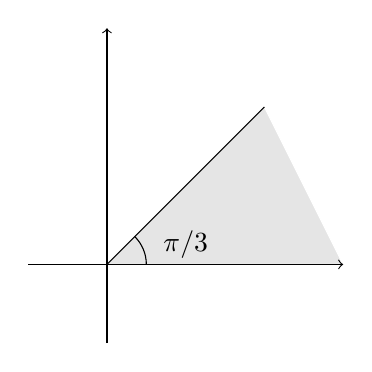
\begin{tikzpicture}
            \filldraw[fill=gray!20,draw=white] (0,0) -- (2,2) -- (3,0) -- (0,0);
            \draw[->] (-1,0) -- (3,0);
            \draw[->] (0,-1) -- (0,3);
            \draw[-] (0,0) -- (2,2);
            \draw (0.5,0) arc (0:45:0.5);
            \node at (1,0.25) {$\pi / 3$};
        \end{tikzpicture}
    };

    \node (c) at (16,0) {
        
\begin{tikzpicture}
            \filldraw[fill=gray!20,draw=white] (-2,0) -- (2,0) -- (2,1) -- (-2,1) -- (-2,0);
            \draw[-] (-2,0) -- (2,0);
        \end{tikzpicture}
    };

    \node (d) at (24,0) {
        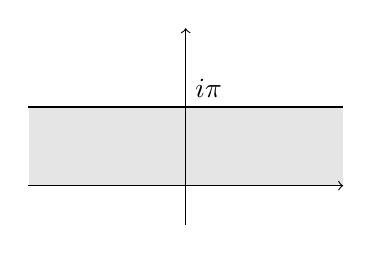
\begin{tikzpicture}
            \filldraw[fill=gray!20,draw=white] (-2,1) rectangle (2,0);
            \draw[->] (-2,0) -- (2,0);
            \draw[->] (0,-0.5) -- (0,2);
            \draw[-] (-2,1) -- (2,1);
            \node[anchor=south west] at (0,1) {$i\pi$};
        \end{tikzpicture}
    };

    \draw[->] (a) -- (b) node[midway,above] {$g(z) = - \dfrac{z+\sqrt{3}}{z-\sqrt{3}}$};
    \draw[->] (a) -- (b) node[midway,below] {$g(i) = - \dfrac{i+\sqrt{3}}{i-\sqrt{3}}$};
    \draw[->] (b) -- (c) node[midway,above] {$z^3$};
    \draw[->] (c) -- (d) node[midway,above] {$\log z$};
\end{tikzpicture}
\end{document}